\documentclass{article}
\usepackage{graphicx}
\usepackage[utf8x]{inputenc}
\usepackage[margin=0.9in]{geometry}

\usepackage{enumitem}
\usepackage{hyperref}
\usepackage{authblk}
\usepackage[british]{babel}
\usepackage{wrapfig}
\usepackage{layout}
\usepackage{algorithm}
\usepackage[noend]{algpseudocode}
\usepackage{graphicx}
\usepackage{caption}
\usepackage{subfig}

\title{Hough Transform}
\author{Neal Bayya, George Tang, \& Neil Thistlethwaite}
\date{November 2018}

\begin{document}

\maketitle

\section{Introduction}

The Hough Transform is a feature-extraction algorithm for identifying shapes in images, classically lines. The general process involves a "vote casting", whereby each edge pixel that is being considered to be part of a shape is allowed to cast "votes" in parameter space. At the end of the process the possible shapes (parameter configurations) with the most votes are considered to be the ones that actually exist in the image. This effectively reduces the problem by allowing possibilities to be checked only once, rather than once for every time a candidate is visited. 

\begin{figure}[!h]
\centering
\begin{minipage}{.5\textwidth}
  \centering
  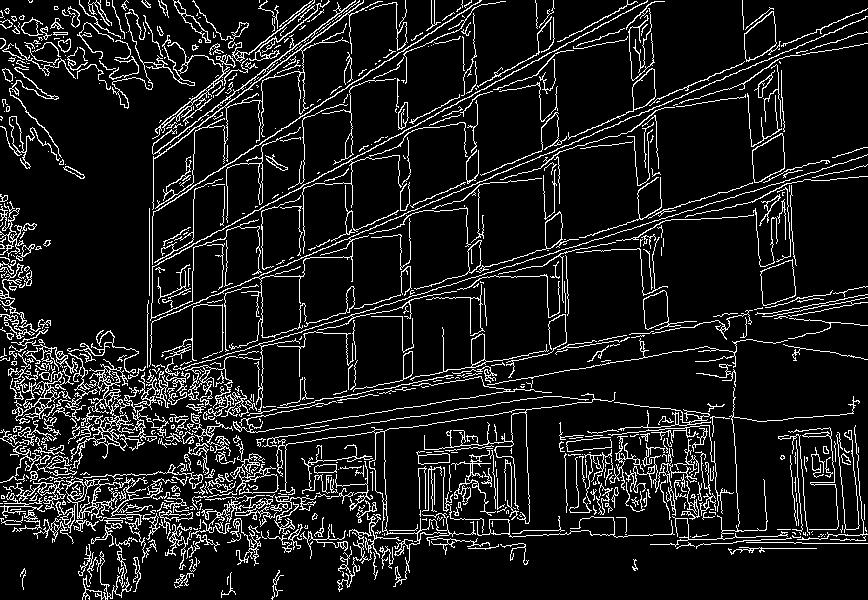
\includegraphics[width=0.7\linewidth]{bld1}
  \captionof{figure}{Original Image}
  \label{fig:test1}
\end{minipage}%
\begin{minipage}{.5\textwidth}
  \centering
  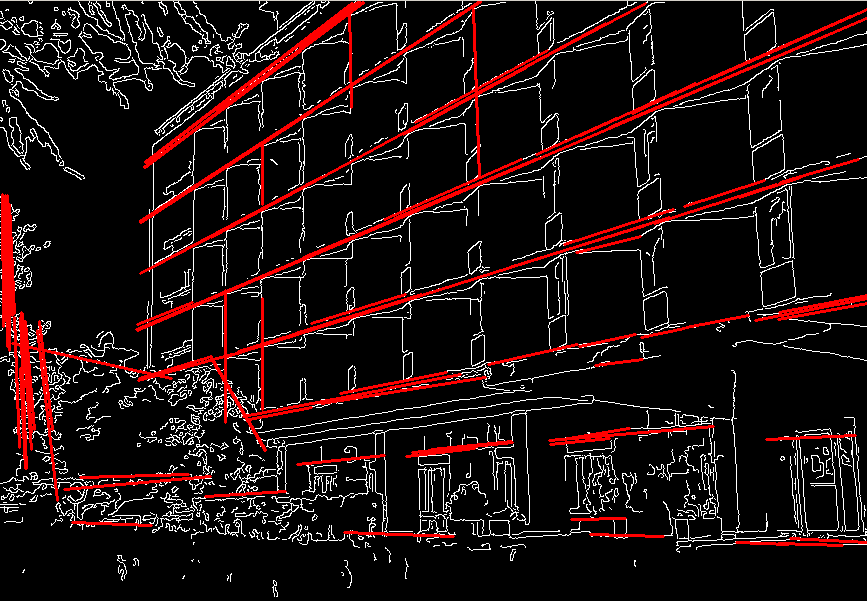
\includegraphics[width=0.7\linewidth]{bld2}
  \captionof{figure}{Lines Detected via Hough Transform}
  \label{fig:test2}
\end{minipage}
\end{figure}

\section{Line Detection}

As an example, let us consider the simple case of line detection. First, we must define our parameter space that the points will vote in. Each point in the parameter space must correspond to a unique line, thus one clear choice would be to represent the lines in slope-intercept form, using \begin{math}(m,c)\end{math} as the parameter space. Interestingly enough, if we draw a line in \begin{math}(m,c)\end{math} for each edge pixel (defined by an x and y), then the intersection will tell us the fit a slope and intercept to the line. Refer to Figure \ref{fig:spaces} for a visualization of line fitting with the $(m,c)$ space. One problem we run into is that the space \begin{math}(m,c)\end{math} is not bounded; near-vertical lines cause the slope to go to infinity. 

\begin{figure}[!h]
    \centering
    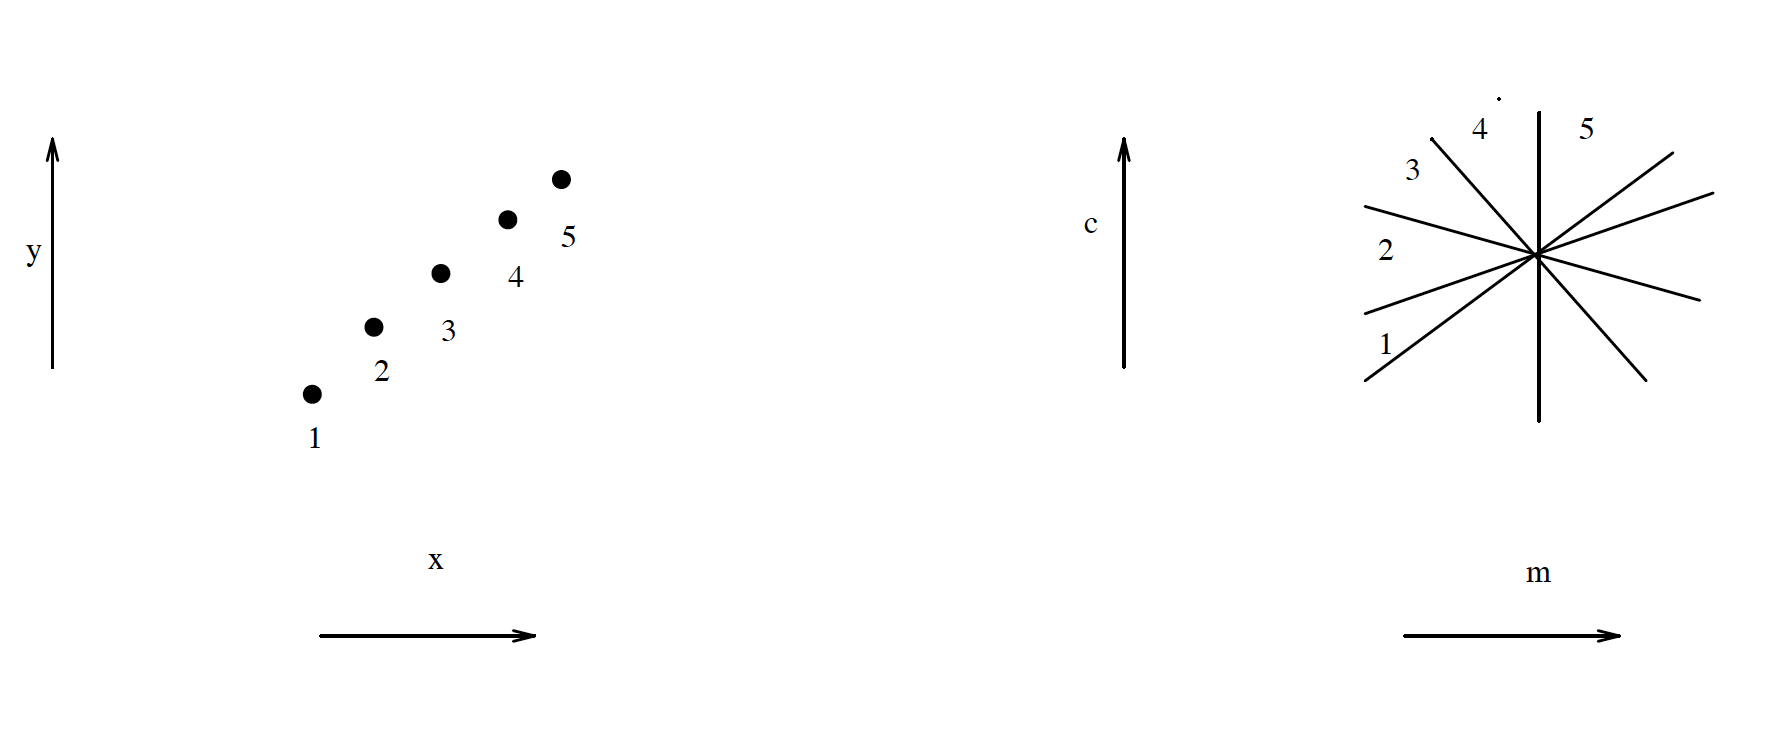
\includegraphics[width=0.8\textwidth]{spaces}
    \caption{Edge pixels of straight line on left each translate to a line in $(m,c)$ space. Lines intersect at one $(m,c)$ coordinate.}
    \label{fig:spaces}
\end{figure}

Our solution for this is to instead use \textit{Hesse normal form}, which expresses a line as a location in 2D space and a direction that the line extends in. Specifically, we use the form
\begin{equation}r=x\cos{\theta}+y\sin{\theta}\end{equation}
Where \begin{math}r\end{math} and \begin{math}\theta\end{math} define the line as shown in Figure \ref{fig:diagram}. That is, to go from a \begin{math}(r,\theta)\end{math} pair to a line, you extend out from the origin r units at an angle of \begin{math}\theta\end{math} above the x axis (shown in blue), then construct the line perpendicular (shown in red). With a little mathematical manipulation, it can be shown that the provided equation does indeed represent the red line. One neat advantage of this representation is that $\theta$ can be computed directly from the gradient angle in edge detection. This reduces the complexity of searching for a fitted line as we no longer have to search over different angles.

\begin{figure}[!h]
    \centering
    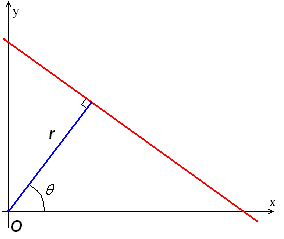
\includegraphics[width=0.25\textwidth]{diagram}
    \caption{Line Representation in \textit{Hesse normal form}}
    \label{fig:diagram}
\end{figure}

\noindent
To perform Hough Transform, we initialize an 2-D accumulator array \begin{math}A[r,\theta]\end{math} in the parameter space. Each edge pixel will cast a number of votes for specific $(r, \theta)$ pairs into the accumulator function to model the line. At the end, the point maxima in the accumulator will represent lines. Since there's an infinite choices for r and $\theta$, we discretize the accumulator by picking a finite number of angles and values of r to consider. In other words, the accumulator array is discretized by making bins of some size when casting votes; this size is usually dependent on and directly relates to the size of the image you are dealing with. Refer to Algorithm \ref{linealgo} for the implementation details of finding the lines in an image using Hough Transform.

\begin{algorithm}
\caption{Hough Transform Line Detection}
\label{linealgo}
\begin{algorithmic}
    \Function{Linear Hough Transform}{}
        \State Initialize an accumulator array in the parameter space \begin{math}A[r,\theta]\end{math}
        \For{each edge point (x,y)}
            \State $\theta \gets arctan(\frac{S_y}{S_x})$
            \Comment{$S_y, S_x$ are gradients in y and x directions}
            \State $r = x\cos{\theta}+y\sin{\theta}$
            \State \begin{math}A[r,\theta] += 1\end{math}
            \Comment{Increment the accumulator}
        \EndFor
        \State Find $r,\theta$ parameters of maxima in A[r, $\theta$]
        \Comment{Numer of maxima corresponds to number of lines}\\
        \Comment{If necessary, monitor which edge pixels contribute to the determined lines}
\EndFunction
\end{algorithmic}
\end{algorithm}

\noindent
Notably, the Hough Transform of a single point is a unique sinusoid in the parameter space, each point along the sinuosoid representing a different line that the point could be a part of. Effectively, our parameter representation has changed the problem of detecting lines into detecting intersection points of sine waves, as the points where many sine functions intersect will be the lines that actually exist in the image. 

\section{Circle Detection}
To deepen our applications of Hough Transform, let's try fitting circles in our image. A circle can be represented by the equation \begin{math}(x-x_0)^2+(y-y_0)^2=r^2\end{math}. Our parameter space would thus be represented by our three unknowns: \begin{math}(x_0,y_0,r)\end{math}. However, we can use $\theta$ from the gradient to reduce the complexity in this case as well. The center location $(x_0,y_0)$ can be computed directly from ($r, \theta$) as ($x-rcos(\theta), y-rsin(\theta)$). Using $\theta$ we only have to search over varying radius sizes. Algorithm \ref{circalgo} outlines Hough Transform for circles.

\begin{algorithm}
\caption{Hough Transform Circle Detection}
\label{circalgo}
\begin{algorithmic}
    \Function{Circle Hough Transform}{}
        \State Initialize an accumulator array in the parameter space $A[x_0,y_0,r]$
        \For{each edge point (x,y)}
            \For{r = $r_{min}$; $r \leq r_{max}$}
                \State $\theta \gets arctan2(S_y, S_x)$
                \Comment{$S_y, S_x$ are gradients in y and x directions}
                \State $x_0 = x-rcos(\theta)$
                \State $y_0 = y-rsin(\theta)$
                \State $A[x_0,y_0,r] += 1$
                \Comment{Increment the accumulator}
            \EndFor
        \EndFor
        \State Find $x_0,y_0,r$ parameters of maxima in $A[x_0,y_0,r]$
        \Comment{maxima corresponds to circles}\\
        \Comment{If necessary, monitor which edge pixels contribute to the determined circles}
\EndFunction
\end{algorithmic}
\end{algorithm}

\begin{figure}[!h]
    \centering
    \vspace{-10pt}
    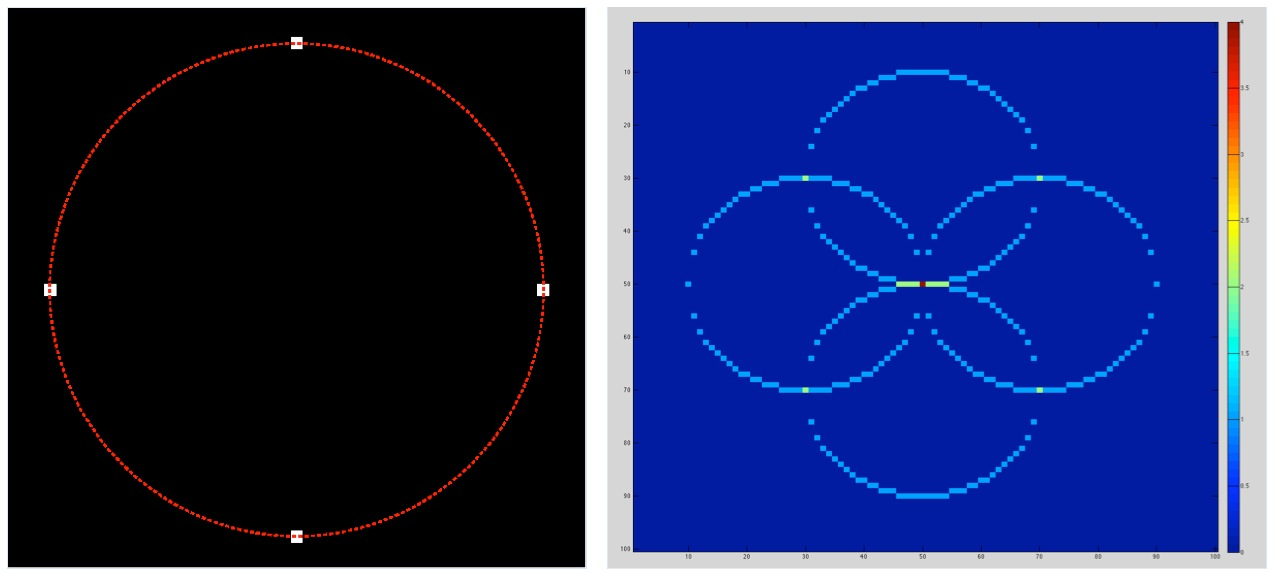
\includegraphics[width=0.8\textwidth]{circle.jpg}
    \caption{Four edge points on a circle processed using Hough Transform}
    \label{fig:diagram}
\end{figure}

\begin{figure}[!h]
    \centering
    \vspace{-10pt}
    \hspace{-30pt}
    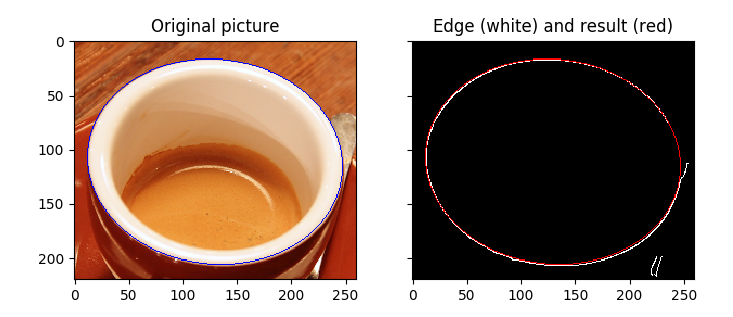
\includegraphics[width=0.8\textwidth]{coffe.png}
    \caption{Hough Transform to detect coffee mug}
    \label{fig:diagram}
\end{figure}

\section{Generalized Shape Detection}
As it turns out, the Hough Transform can be generalized for detecting any parameterizable shape in an image. The key is choosing a well-defined parameter space (for instance, without any of the infinite discontinuities in the \begin{math}(m,b)\end{math} parameterization of lines). Using these steps,you can easily fit edges to complex shapes such as ellipses. Algorithm \ref{genalgo} outlines the general procedure for applying Hough to various analytical shapes.

\begin{algorithm}
\caption{General Hough Transform Detection}
\label{genalgo}
\begin{algorithmic}
    \Function{General Hough Transform}{}
        \State Define parameter space $P$
        \State Initialize an accumulator array in the parameter space $A[P]$
        \For{each edge point (x,y)}
            \For{$p_1$ = $p_{1min}$; $p_1 \leq p_{1max}$}
                \For {$p_2$ = $p_{2min}$; $p_2 \leq p_{2max}$} \\
                    \State ...
                    \Comment{Nest for loops until all parameters can be identified}
                    \State Find parameter values ${p_1, p_2, p_3,... p_n}$ from $x,y$ and the iterated variables
                    \State $A[p_1, p_2, p_3,... p_n] += 1$
                    \Comment{Increment the accumulator}
                \EndFor
            \EndFor
        \EndFor
        \State Find $p_1, p_2, p_3,... p_n$ parameters of maxima in $A[P]$
\EndFunction
\end{algorithmic}
\end{algorithm}

\section{Shape Constraints}
It is also possible to set constraints on the shape that the Hough Transform detects. For instance, in the example of circles, suppose we only wanted to detect circles with a diameter between 30 pixels and 50 pixels. We can impose this constraint by simply restricting the domain of \begin{math}r\end{math} in the accumulator to \begin{math}[30, 50]\end{math}. Anything outside will not be incremented (or iterated through in the innermost loop). Likewise, we could impose a constraint on \begin{math}\theta\end{math} in the line detection example if we only wanted to detect lines in certain directions. 

\section{Summary}
The Hough Transform is a powerful and robust algorithm for shape detection when \textit{you know what you're looking for}, with many applications from something as contrived as detecting the rungs of a ladder to detecting street signs or markings on the road in an autonomous vehicle. 
\end{document}